%----------------------------------------------------------------------
%	REQUIRED PACKAGES
%----------------------------------------------------------------------
\documentclass[12pt]{report}
\usepackage[numbers,sort&compress]{natbib}
\usepackage[utf8]{inputenc}
\usepackage{amsmath,amsfonts,amssymb}
\usepackage{graphicx}
\usepackage{tikz}
\usepackage{float}
\usepackage{placeins}
\usepackage{url}
\usepackage{caption}
\usepackage{setspace}
\usepackage{tocloft}

%----------------------------------------------------------------------
%	FONTS,INDENTATION, MARGINS, LINE SPACING
%----------------------------------------------------------------------
\usepackage{times}      % Loads the Times-Roman Fonts
\usepackage{mathptmx}   % Loads the Times-Roman Math Fonts
\usepackage[left=3.81cm,
            right=2.54cm,
        top=2.54cm,
        bottom=2.54cm,
        a4paper]{geometry}
  
\setlength{\parindent}{0pt} % Remove paragraph indent globally
\usepackage{setspace} %package for line spacing
\setstretch{1.5}
\usepackage{parskip}
\setlength{\parskip}{6pt}  % Adjust paragraph spacing as needed

%----------------------------------------------------------------------
%	TITLES,SECTIONS,SUBSECTIONS AND SUBSUBSECTIONS
%----------------------------------------------------------------------
\usepackage{titlesec}
\titlespacing{\chapter}{0pt}{-24pt}{12pt}
\titlespacing{\section}{0pt}{16pt}{16pt}
\titlespacing{\subsection}{0pt}{16pt}{16pt}
\titlespacing{\subsubsection}{0pt}{16pt}{16pt}

\titleformat{\chapter}[display]{\centering\fontsize{14pt}{12pt}\bfseries}{\MakeUppercase{\chaptertitlename\ \thechapter}}{12pt}{}
\titleformat{\section}{\fontsize{12pt}{16pt}\bfseries\raggedright}{\thesection}{0.5em}{}
\titleformat{\subsection}{\fontsize{12pt}{16pt}\bfseries\raggedright}{\thesubsection}{0.5em}{}
\titleformat{\subsubsection}{\fontsize{12pt}{16pt}\bfseries\raggedright}{\thesubsubsection}{0.5em}{}
\titleformat{\paragraph}{\fontsize{12pt}{0pt}\bfseries\raggedright}{\theparagraph}{0.5em}{}

%----------------------------------------------------------------------
%	FORMATTING THE TABLE OF CONTENTS,LOF AND LOT
%----------------------------------------------------------------------

% Adjust the spacing for the TABLE OF CONTENT
\renewcommand{\cftbeforetoctitleskip}{-18pt} % Space before the TOC title
\renewcommand{\cftaftertoctitleskip}{12pt} % Space after the TOC title
\renewcommand{\cftbeforechapskip}{9pt} % Space before each chapter entry
\renewcommand{\cftbeforesecskip}{9pt} % Space before each section entry
\renewcommand{\cftbeforesubsecskip}{9pt} % Space before each section entry
\renewcommand{\contentsname}{\fontsize{14}{16}\bfseries TABLE OF CONTENTS}

% Adjust the spacing for the LIST OF FIGURES
\renewcommand{\cftbeforeloftitleskip}{-18pt} % Space before the LOF title
\renewcommand{\cftafterloftitleskip}{12pt} % Space after the LOF title
\renewcommand{\cftbeforefigskip}{10pt} % Space before each figure entry
\renewcommand{\listfigurename}{\fontsize{14}{16}\bfseries LIST OF FIGURES}
\renewcommand{\cftfigpresnum}{\figurename\ }
\renewcommand{\cftfigaftersnum}{:}
\renewcommand{\cftfigaftersnumb}{\hspace{2.5em}} 

% Adjust the spacing for the LIST OF TABLES
\renewcommand{\cftbeforelottitleskip}{-18pt} % Space before the LOT title
\renewcommand{\cftafterlottitleskip}{12pt} % Space after the LOT title
\renewcommand{\cftbeforetabskip}{10pt} % Space before each table entry
\renewcommand{\listtablename}{\fontsize{14}{16}\bfseries LIST OF TABLES}
\renewcommand{\cfttabpresnum}{Table\ }
\renewcommand{\cfttabaftersnum}{:}
\renewcommand{\cfttabaftersnumb}{\hspace{2.5em}}

%----------------------------------------------------------------------
%	HYPERLINKS CONFIGURATION
%----------------------------------------------------------------------
% hyperref should be the last package loaded
\usepackage[pdftex,
            colorlinks=true,
            linkcolor=black,
            citecolor=black,
            urlcolor=black,
            bookmarks=true,
            bookmarksopen=true,
            bookmarksnumbered=true,
            pdfborder={0 0 0},
            breaklinks=true,
            pdftitle={Campus Connect: A Student Information System},
            pdfauthor={Student Name}]{hyperref}

%----------------------------------------------------------------------
%	END OF PREAMLBE AND BEGINNING OF THE DOCUMENT
%----------------------------------------------------------------------

\begin{document}

\pagenumbering{roman} % roman page numbers
\begin{titlepage}
    \centering
    
    
\includegraphics[width=0.2\textwidth]{Graphics/TULogo.png}\par
    \vspace{1.2cm}
    {\fontsize{14pt}{12pt}\selectfont\textcolor{black}
    TRIBHUVAN UNIVERSITY \par INSTITUTE OF ENGINEERING \par PURWANCHAL CAMPUS \par
    \vspace{1.2cm}
    \begin{flushleft}
    
    \end{flushleft}

    % {\bfseries\textcolor{black}
    \par A MINOR PROJECT PROPOSAL ON PROJECT TITLE \par

    \vspace{1.2cm}
    BY\par SANGYOG PURI (PUR078BCT078)
      \par SANSKAR RIJAL (PUR078BCT079)
      \par SUJAN NAINAWASTI (PUR078BCT090)
      \par VISION PEER CHAUDHARY (PUR078BCT094)
    \par
    \vspace{1.2cm}\par
    }
    {\fontsize{13pt}{12pt}\selectfont\textcolor{black}
    DEPARTMENT OF ELECTRONICS AND COMPUTER ENGINEERING\par PURWANCHAL CAMPUS\par DHARAN, NEPAL\par
    \vspace{1.2cm}
    \vspace{1.2cm}
    
    DECEMBER, 2024 
    }
\end{titlepage}


%\pagenumbering{roman} % roman page numbers
\begin{titlepage}
    \centering
    
    {\fontsize{12pt}{14pt}\bfseries\textcolor{black}{PROJECT TITLE GOES HERE}\par}
    \vspace{2.0cm}
       {By} \par {STUDENT NAME}({ROLL NUMBER})
            \par {STUDENT NAME}({ROLL NUMBER})
            \par {STUDENT NAME}({ROLL NUMBER})
            \par {STUDENT NAME}({ROLL NUMBER})
       \vspace{2.0cm}\par
    Project Supervisor\par
    Asst. Prof. Pukar Karki\par
    \vspace{2.0cm}
    {A project submitted to the Department of Electronics and Computer Engineering in partial fulfillment of the requirements for the Bachelor’s Degree in Computer Engineering}\par
        \vspace{2.0cm}\par

    {Department of Electronics and Computer Engineering\\ Purwanchal Campus, Institute of Engineering \\ Tribhuvan University\\ Dharan, Nepal}\par
        \vspace{2.0cm}\par
        
   {January , 2024}
   
\end{titlepage}




%\include{Copyright}
%\include{Declaration}
%\chapter*{Recommendation}
\addcontentsline{toc}{chapter}{Recommendation}
The undersigned certify that they have read and recommended to the Department of
Electronics and Computer Engineering for acceptance, a project entitled \textbf{``PROJECT NAME GOES HERE"}, submitted by \textbf{STUDENTS NAME} in partial fulfillment of the requirement for the award of the degree of \textbf{``Bachelor of Engineering in Computer Engineering"}.\par
        \vspace{1cm}
..........................................................................\\
\textbf{Asst. Prof. Pukar Karki\\
Supervisor\\
Department of Electronics and Computer Engineering\\
Purwanchal Campus, Institute of Engineering, Tribhuvan University}\par
        \vspace{1cm}
..........................................................................\\
\textbf{Prof. Subarna Shakya, (PhD)\\
External Examiner \\
Department of Electronics and Computer Engineering\\
Pulchowk Campus, Institute of Engineering, Tribhuvan University}\par
        \vspace{1cm}
..........................................................................\\
\textbf{
Asst. Prof. Pravin Sangroula\\ 
Head of Department \\
Department of Electronics and Computer Engineering\\Purwanchal Campus, Institute of Engineering, Tribhuvan University}\par
\vspace{2.5cm}

\begin{center}
\textbf{10\textsuperscript{th} January, 2024}
\end{center}
\newpage


%\include{DeptAcceptance}
\chapter*{ACKNOWLEDGEMENT} \addcontentsline{toc}{chapter}{ACKNOWLEDGEMENT}

We are very thankful to the Department of Electronics and Computer Engineering for providing this opportunity. It has been a greatly endearing experience.

We would like to express our deepest gratitude to our esteemed supervisor, Asst. Prof. Prasanga Regmi, for his invaluable guidance and support throughout the project.

Additionally, we would like to express our appreciation to Deputy Head of Department (HOD) Pukar Karki for routinely checking on us and ensuring the progress of the project.

We would also like to acknowledge the support and mentorship provided by our seniors, for their insightful suggestions, constructive feedback, and generous allocation of time and resources toward the successful completion of our project.

We extend our special thanks to Mr. Sujan Karki for his assistance in reviewing our final documents, which greatly improved the quality of our work.

\vspace{1cm} Sincerely,\\ Sangyoug Puri\\ Sanskar Rijal\\ Sujan Nainawasti\\ Vision Peer Chaudhary
\chapter*{ABSTRACT} \addcontentsline{toc}{chapter}{ABSTRACT}

The Institute of Engineering (IOE) in Nepal currently utilizes various disparate platforms for providing services to its students and staff. Campus Connect is being developed as a comprehensive platform with a user-friendly interface integrating all services in one place. This platform aims to integrate existing services while providing additional features through the use of plugin-like technology. The Campus Connect app strives to provide seamless services to its users and enhance the efficiency and centralization of college activities. The Agile methodology approach has been adopted to ensure that Campus Connect meets the requirements of its target audience. Furthermore, the Campus Connect's monolithic architecture allows for simplistic and cost-effective services, which can pave the way for similar applications to be developed for other educational organizations.

\vspace{1cm} Keywords: \textit{IOE, Nepal, platform, Agile methodology, monolithic architecture}
{\centering{\tableofcontents}}\newpage
{\centering\listoffigures\addcontentsline{toc}{chapter}{LIST OF FIGURES}}
\newpage

\newpage
\chapter*{LIST OF ABBREVIATIONS}
% \vspace{1cm}
\addcontentsline{toc}{chapter}{LIST OF ABBREVIATIONS}
\begin{tabular}{l l}
API	&	:	Application Programming Interface	\\
Colab	&	:	Colaboratory	\\
REST	&	:	Representational State Transfer	\\
IOE	&	:	Institute Of Engineering	\\
IOEPC	&	:	Institute Of Engineering Purwanchal Campus	\\
MVVM	&	:	Model-View-ViewModel	\\
 


\end{tabular}









\pagenumbering{arabic}
\chapter{Introduction}

\section{Background}
The Institute of Engineering Purwanchal Campus (IOEPC) is the leading technical education institution in Nepal and offers undergraduate and graduate programs in various fields of engineering, such as civil engineering, mechanical engineering, electrical engineering, electronics and communication engineering, computer engineering, and architecture. It currently carries out administrative and academic tasks both offline and online. While most academic notices are published through social media, including daily routines, this causes important notices to be missed and reliance on third-party software. Moreover, there is a lack of a centralized website or application to access all college-related work. To address this, we propose the development of a mobile application that can integrate all college services and is flexible for future enhancements. Our aim is to provide a convenient and efficient platform for college students while ensuring easy integration of existing offline processes. We anticipate that this application will be highly advantageous to the Institute of Engineering.

\section{Gap Identification}
\begin{itemize}
    \item The current services of IOEPC are mostly manual and offline, leading to delays and inefficiencies.
    \item The current system lacks real-time updates and fails to provide timely and relevant information to students; the class schedule is heavily reliant on the class representative.
    \item Dependency on social media causes some important notices, like late fee notices, to be missed.
    \item The library management is not integrated and is run separately.
    \item A modernized system, such as a mobile app, is needed to provide a centralized platform for communication, access to course materials, and other relevant resources.
\end{itemize}

\section{Motivation}
The Campus Connect app is inspired by the difficulties we faced during our time in college. The inconsistencies between the services provided by the campus and their accessibility have been the driving force. A student isn’t aware when fee notices are published if they don’t come across a specific Facebook post. Teachers canceling classes at the last minute, while failing to convey it to the class representative, causes commuting students hassle.

\section{Objectives}
\begin{itemize}
    \item To create an easily scalable and integrable college application.
    \item To improve online access to the educational system and mitigate current problems by using monolithic architecture.
\end{itemize}
\chapter{RELATED THEORY}
\section{Related Theory goes here}




\chapter{Literature Review}

\section{Introduction}
The literature review provides an overview of existing research and developments related to the proposed mobile application for the Institute of Engineering Purwanchal Campus (IOEPC). This section examines previous studies on mobile application development, monolithic architecture, and the use of React/React Native and Kotlin, highlighting the gaps and opportunities that the proposed project aims to address.

\section{Mobile Application Development}
Previous research has extensively explored the principles and practices of mobile application development. Smith (2020) discusses the importance of user-centered design and the need for seamless integration between frontend and backend components. However, there is limited research on the specific challenges faced by educational institutions in developing mobile applications tailored to their unique needs.

\section{Monolithic Architecture}
Johnson (2019) provides a comprehensive overview of monolithic architecture, emphasizing its simplicity and ease of deployment. While this approach is well-suited for small to medium-sized applications, there is a need for further research on its scalability and maintainability in the context of educational applications.

\section{React/React Native}
Brown (2018) highlights the advantages of using React and React Native for building responsive and interactive user interfaces. These technologies have been widely adopted in various industries, but their application in educational settings remains underexplored. The proposed project aims to leverage these technologies to create a user-friendly admin panel for IOEPC.

\section{Kotlin}
Lee (2021) discusses the benefits of using Kotlin for Android development, including its concise syntax and improved safety features. While Kotlin has gained popularity among developers, there is limited research on its use in developing educational applications. The proposed project will utilize Kotlin to develop the student and teacher portals, addressing this gap in the literature.

\section{Conclusion}
The literature review highlights the existing research and developments related to the proposed project, identifying gaps and opportunities for further exploration. By building on the insights gained from previous studies, the proposed mobile application aims to provide a comprehensive and user-friendly solution for IOEPC.
\chapter{METHODOLOGY}

\section{Overview}
The development of this project follows an Agile Development Model, ensuring continuous feedback and iterative improvements. The system is built using a Monolithic Architecture, integrating all components into a single unified application. This structure allows seamless communication between different system modules, improving efficiency and maintainability.

The project is developed using:
\begin{itemize}
    \item \textbf{Front-end:} React (for web) and Kotlin (for mobile).
    \item \textbf{Back-end:} Node.js with PostgreSQL as the database.
    \item \textbf{Version Control:} GitHub and Git tools were used for tracking changes and collaboration.
    \item \textbf{Deployment:} The system is hosted on Azure and Vercel to ensure scalability and high availability.
\end{itemize}

\section{Requirement Analysis}
To ensure the system meets the needs of students, teachers, and administrators, a requirement analysis phase was conducted. This involved:
\begin{itemize}
    \item \textbf{User Interviews:} Discussions with students and faculty members to identify key functionalities.
    \item \textbf{Comparative Analysis:} Reviewing existing educational management systems to understand their strengths and weaknesses.
\end{itemize}

Key requirements derived from this phase include:
\begin{itemize}
    \item A student dashboard for accessing attendance, marks, and notices.
    \item A teacher dashboard for managing attendance and internal assessments.
    \item An admin panel for user account management.
\end{itemize}

\section{System Architecture}
The system is developed using a Monolithic Architecture, where all functionalities are integrated into a single codebase. This approach simplifies development, deployment, and maintenance.

\subsection{Architecture Components}
\begin{itemize}
    \item \textbf{Front-end (React \& Kotlin)}
        \begin{itemize}
            \item React is used for the web interface.
            \item Kotlin is used for Android-based mobile applications.
        \end{itemize}
    \item \textbf{Back-end (Node.js \& PostgreSQL)}
        \begin{itemize}
            \item Node.js handles API requests and server-side processing.
            \item PostgreSQL is used as the database to store structured data.
        \end{itemize}
    \item \textbf{Deployment}
        \begin{itemize}
            \item Azure for cloud hosting.
            \item Vercel for front-end deployment.
        \end{itemize}
\end{itemize}

\section{Development Methodology}
The project follows an Agile Development Model, explicitly incorporating:
\begin{itemize}
    \item \textbf{Sprint-Based Development:} The development cycle is divided into multiple sprints, each lasting two weeks.
    \item \textbf{Daily Stand-up Meetings:} To discuss progress, challenges, and next steps.
    \item \textbf{Iterative Feedback:} Testing and improvements after each sprint cycle.
\end{itemize}

\subsection{Sprint Breakdown Example}
\begin{itemize}
    \item \textbf{Sprint 1:} Set up project repository, database schema, and authentication module.
    \item \textbf{Sprint 2:} Develop student dashboard and implement attendance tracking.
    \item \textbf{Sprint 3:} Complete teacher and admin functionalities.
    \item \textbf{Sprint 4:} Testing, debugging, and final deployment.
\end{itemize}

\section{Implementation Strategy}
The system is implemented in three key phases:

\subsection{Front-End Development}
\begin{itemize}
    \item React is used to build reusable UI components for web applications.
    \item Kotlin is used for mobile development to ensure a smooth user experience.
    \item State Management is handled using Redux for React applications.
\end{itemize}

\subsection{Back-End Development}
\begin{itemize}
    \item Node.js with Express manages API requests and business logic.
    \item REST API Architecture is used for communication between the front-end and back-end.
\end{itemize}

\subsection{Database Management}
\begin{itemize}
    \item PostgreSQL stores user data, academic records, and attendance.
\end{itemize}

\section{Testing and Validation}
Testing was conducted to identify usability issues and ensure system reliability. The testing approach included:
\begin{itemize}
    \item \textbf{Unit Testing:} Each component was individually tested using Jest (for Node.js).
    \item \textbf{Integration Testing:} API endpoints were tested using Postman to ensure smooth communication.
    \item \textbf{User Acceptance Testing (UAT):} A group of students and teachers used the system and provided feedback.
\end{itemize}

\section{Deployment and Maintenance}
\begin{itemize}
    \item \textbf{Hosting Platforms:}
        \begin{itemize}
            \item Azure is used for cloud hosting of the back-end.
            \item Vercel is used for front-end deployment.
        \end{itemize}
    \item \textbf{Version Control \& CI/CD:}
        \begin{itemize}
            \item GitHub \& Git tools are used for source code management.
            \item Continuous Integration (CI) is implemented to automate testing and deployment.
        \end{itemize}
    \item \textbf{Future Maintenance:}
        \begin{itemize}
            \item Regular updates based on user feedback.
            \item Bug fixes and feature enhancements will be tracked using GitHub Issues.
        \end{itemize}
\end{itemize}
\chapter{SYSTEMDESIGN}
\section{Overview}
\section{Other section goes here}




\chapter{TECHNOLOGY USED}

\section{Front-End}

\subsection{React}
React, an open-source project developed by Meta, is a JavaScript library that permits developers to create an interactive user interface for web applications. It helps in simplifying the building of complex user interfaces. The major work of React involves breaking down the UI into reusable components that are then utilized to construct the more complex UI elements. It supports code reusability and makes the use of state changes easier within the application. In React, there is the virtual DOM whose implementation helps to improve the time and performance for rendering the content in DOM \cite{react2025}.

\subsection{TypeScript}
To add the optional static typing to the language, a superset of JavaScript is used which is known as TypeScript. It is better known to improve code quality and maintainability by catching the bugs at the time of compiling. It comprises several features like auto-completion, code navigation, and helping to prevent common errors during programming. With the help of TypeScript, the developers write more maintainable and scalable code creating a better user experience for their applications \cite{typescript2025}.

\subsection{Kotlin}
Kotlin, developed by JetBrains, is a statically typed programming language that is fully interoperable with Java. It features a concise syntax, reducing boilerplate code, and introduces null safety to prevent common null pointer exceptions. With smart casts, extension functions, and built-in support for asynchronous programming via coroutines, Kotlin provides a modern and efficient coding experience. It is widely adopted for Android development due to its compatibility with Java and its advanced features \cite{kotlin2025}.

\section{Back-End}

\subsection{Node.js}
Node.js is a popular and powerful backend framework that enables developers to build fast, scalable, and event-driven applications using JavaScript. It’s known for its efficient I/O operations, non-blocking I/O model, and a vast library of modules and packages via its package manager, npm. Node.js is also flexible and easy to learn, thanks to its JavaScript syntax and supportive community. With Node.js, developers can build robust and high-performance backend systems for web and mobile applications alike \cite{casciaro2020nodejs}.

\subsection{PostgreSQL}
PostgreSQL is widely used by organizations of all sizes for storing and managing their data. It is a powerful, free, and open-source database management system known for its ability to handle complex transactions and robust security features. Developers can extend and customize PostgreSQL to match their specific needs. It is a reliable database solution that is beneficial for any organization intending to store and manage their data efficiently.
\chapter{OUTPUT}

\section{Attendance Tab}
The attendance service is a crucial feature of the app that allows students to view their attendance records and teachers to take attendance for their classes. The app enables teachers to take attendance through their mobile devices, and students to view their attendance records in real-time.

\section{Internal Marks Submission Tab}
The internal mark submission feature allows students to submit their marks for internal assessment, and teachers to access and manage the marks of their students. The app has a user-friendly interface that allows students and teachers to upload and view the marks easily.

\section{Result Section}
The result section of the app allows students to view their examination results. The app retrieves the result data from the database and displays it in an organized way, such as using a table or graph, and provides options for students to filter and search their results based on their courses, semesters, and other relevant criteria.

\section{Notice Page}
The notice page displays important notices published by the teacher, such as daily routine, class cancellation, notes update, and other relevant information. The app allows users to view the notices in a list or grid format and provides options to filter and search the notices based on their categories and tags.

\section{Notes Page}
Teachers can post their notes into the application, and students can view and download the notes through the mobile app. Students can either type down the notes or upload them. The notes will be visible to students for only one semester.

\section{Application Screenshots}

\subsection{Login Interface}
\begin{figure}[H]
    \centering
    
\includegraphics[width=0.5\textwidth]{Graphics/output/login_page.jpg}
    \caption{Login Page for Campus Connect}
    \label{fig:login_page}
\end{figure}

\subsection{Teacher Application}

\begin{figure}[H]
    \centering
    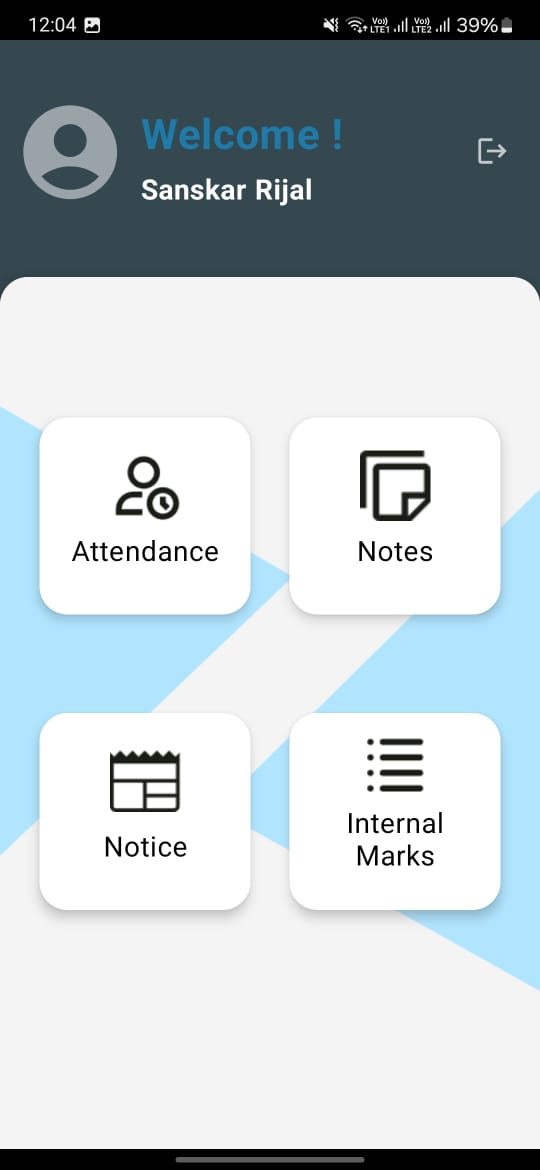
\includegraphics[width=0.5\textwidth]{Graphics/output/teacher_dashboard.jpg}
    \caption{Teacher Dashboard}
    \label{fig:teacher_dashboard}
\end{figure}

\begin{figure}[H]
    \centering
    
\includegraphics[width=0.5\textwidth]{Graphics/output/teacher_subjects.jpg}
    \caption{Subjects Added by Teacher}
    \label{fig:teacher_subjects}
\end{figure}

\begin{figure}[H]
    \centering
    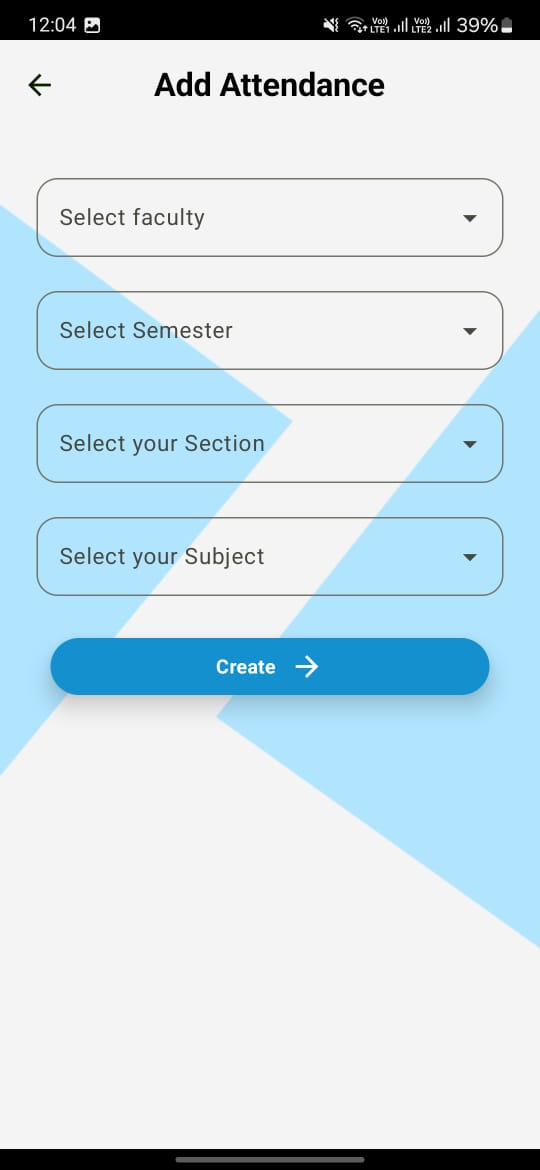
\includegraphics[width=0.5\textwidth]{Graphics/output/teacher_add_subject.jpg}
    \caption{Teacher Adding New Subject}
    \label{fig:teacher_add_subject}
\end{figure}

\begin{figure}[H]
    \centering
    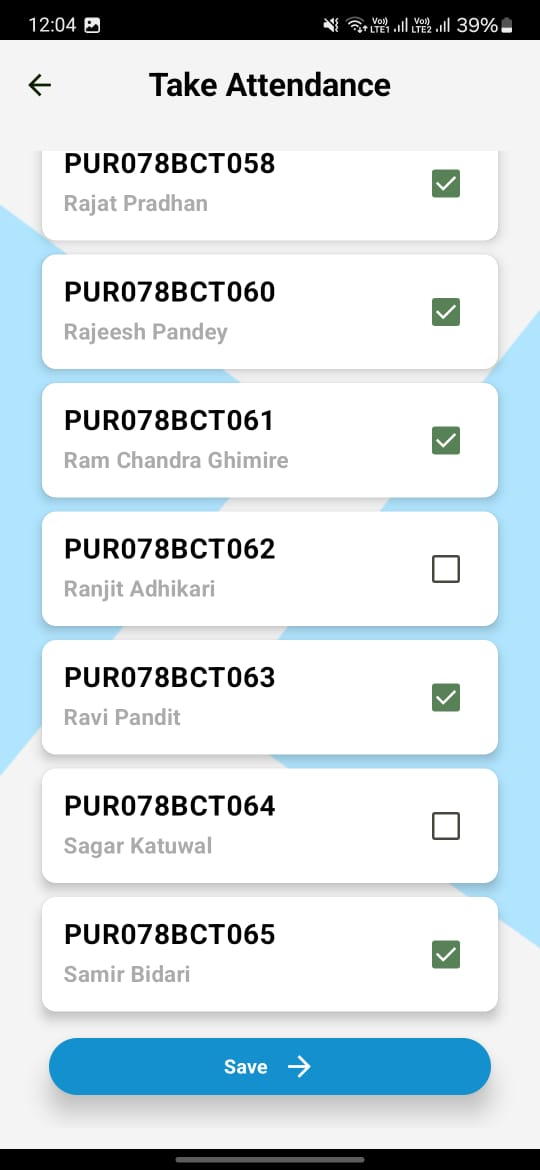
\includegraphics[width=0.5\textwidth]{Graphics/output/teacher_take_attendance.jpg}
    \caption{Teacher Taking Attendance}
    \label{fig:teacher_take_attendance}
\end{figure}

\begin{figure}[H]
    \centering
    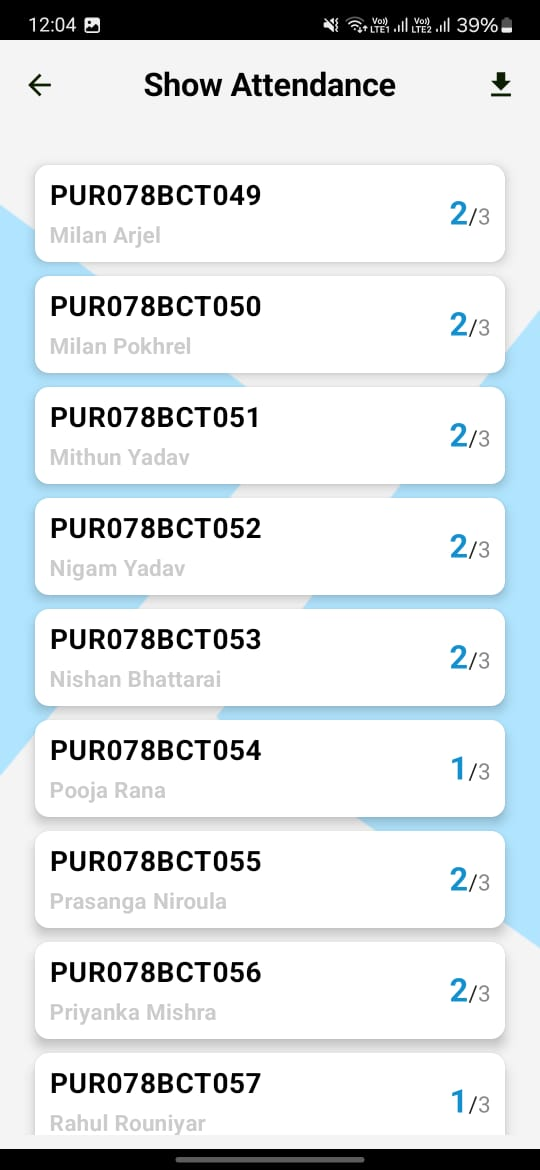
\includegraphics[width=0.5\textwidth]{Graphics/output/teacher_show_attendance.jpg}
    \caption{Teacher Viewing Attendance Records}
    \label{fig:teacher_show_attendance}
\end{figure}

\begin{figure}[H]
    \centering
    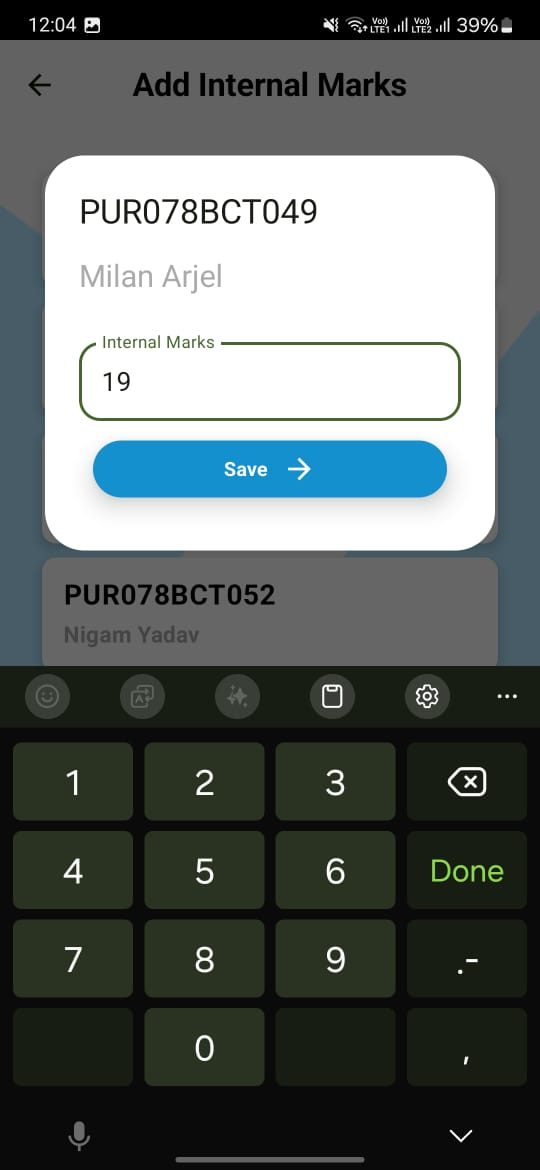
\includegraphics[width=0.5\textwidth]{Graphics/output/teacher_add_marks.jpg}
    \caption{Teacher Adding Internal Marks}
    \label{fig:teacher_add_marks}
\end{figure}

\begin{figure}[H]
    \centering
    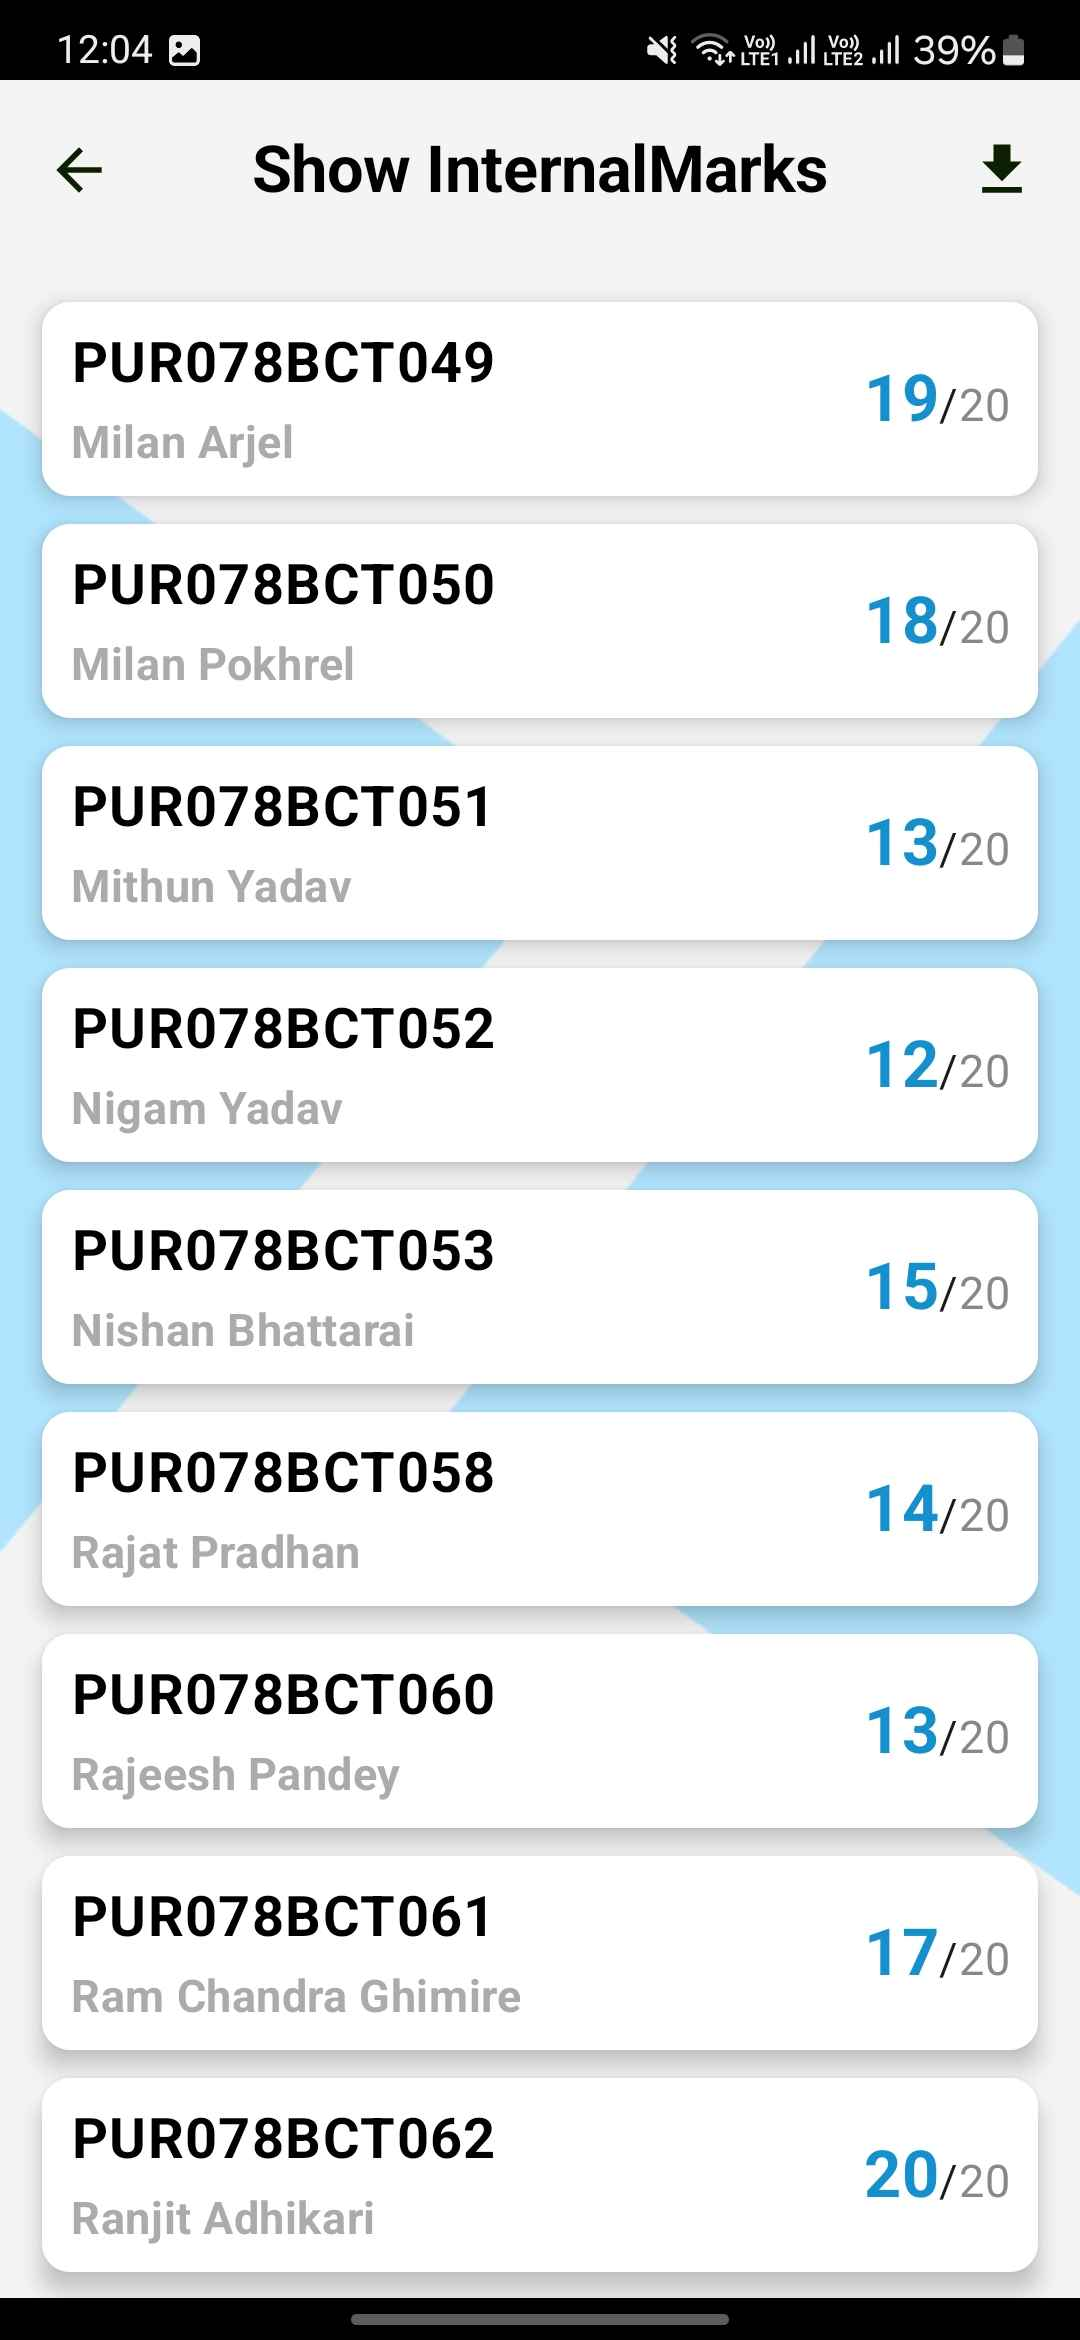
\includegraphics[width=0.5\textwidth]{Graphics/output/teacher_show_marks.jpg}
    \caption{Teacher Viewing Internal Marks}
    \label{fig:teacher_show_marks}
\end{figure}

\begin{figure}[H]
    \centering
    
\includegraphics[width=0.5\textwidth]{Graphics/output/teacher_add_notice.jpg}
    \caption{Teacher Adding Notice}
    \label{fig:teacher_add_notice}
\end{figure}

\begin{figure}[H]
    \centering
    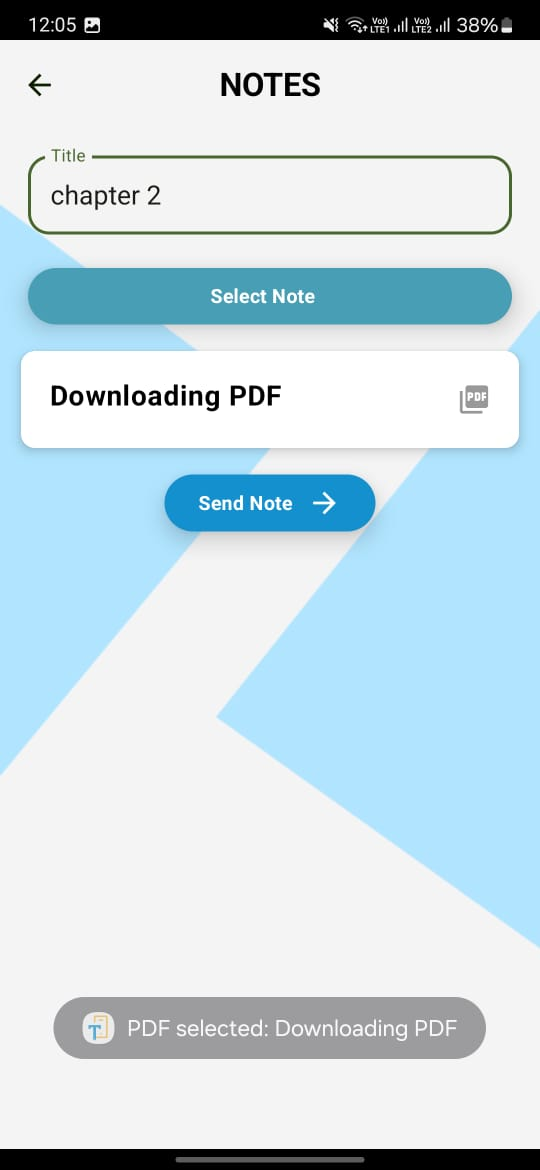
\includegraphics[width=0.5\textwidth]{Graphics/output/teacher_add_notes.jpg}
    \caption{Teacher Adding Notes}
    \label{fig:teacher_add_notes}
\end{figure}

\subsection{Student Application}

\begin{figure}[H]
    \centering
    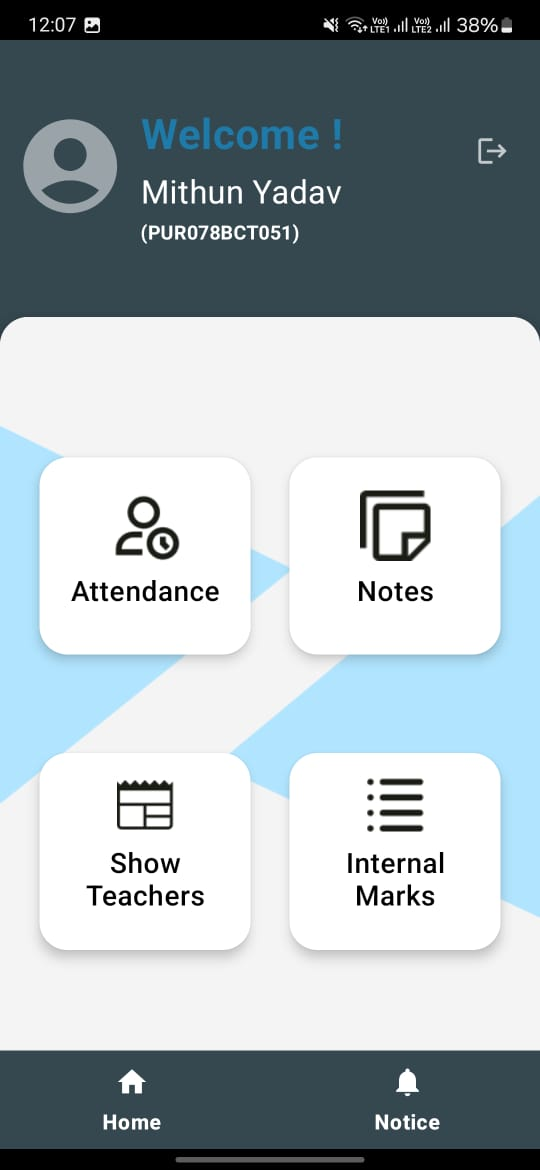
\includegraphics[width=0.5\textwidth]{Graphics/output/student_dashboard.jpg}
    \caption{Student Dashboard}
    \label{fig:student_dashboard}
\end{figure}

\begin{figure}[H]
    \centering
    
\includegraphics[width=0.5\textwidth]{Graphics/output/student_attendance.jpg}
    \caption{Student Viewing Attendance}
    \label{fig:student_attendance}
\end{figure}

\begin{figure}[H]
    \centering
    
\includegraphics[width=0.5\textwidth]{Graphics/output/student_marks.jpg}
    \caption{Student Viewing Internal Marks}
    \label{fig:student_marks}
\end{figure}

\begin{figure}[H]
    \centering
    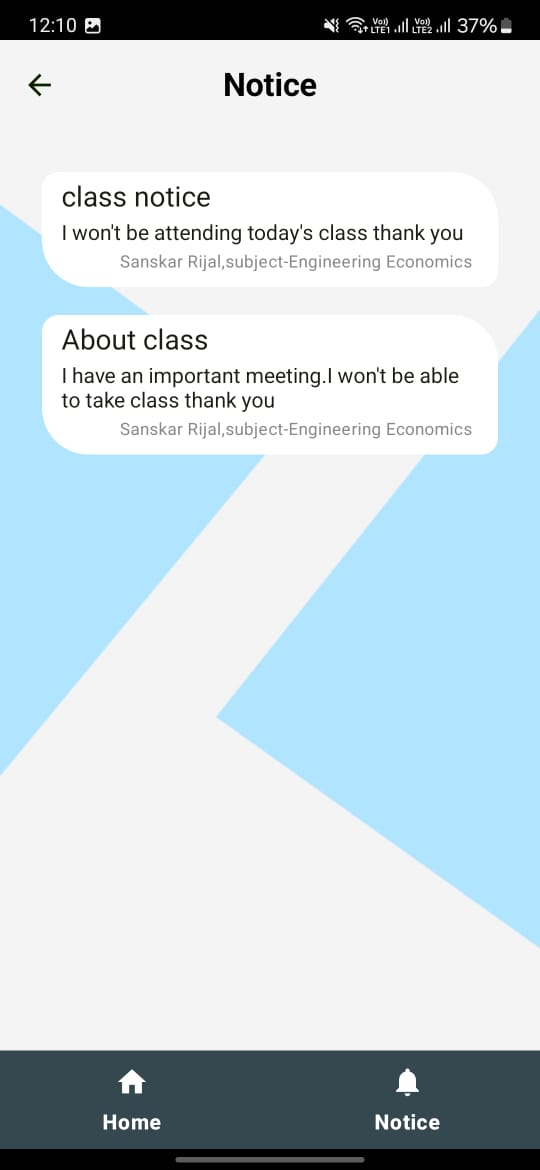
\includegraphics[width=0.5\textwidth]{Graphics/output/student_notices.jpg}
    \caption{Student Viewing Notices}
    \label{fig:student_notices}
\end{figure}

\begin{figure}[H]
    \centering
    
\includegraphics[width=0.5\textwidth]{Graphics/output/student_notes.jpg}
    \caption{Student Accessing Notes}
    \label{fig:student_notes}
\end{figure}

\begin{figure}[H]
    \centering
    
\includegraphics[width=0.5\textwidth]{Graphics/output/student_view_teachers.jpg}
    \caption{Student Viewing Teacher Information}
    \label{fig:student_view_teachers}
\end{figure}

\section{Summary}
The screenshots above demonstrate the key features of the Campus Connect application, providing an efficient way for students to access academic information and for teachers to manage course content, attendance, and assessments.
\chapter{CONCLUSION}

In conclusion, the Campus Connect project has been developed and implemented to provide the Institute of Engineering with an integrated application through which all the activities of the campus can be tracked. It helps students to get easy access to academic information and resources. The app has a user-friendly interface, which allows students to quickly find important information, such as schedules, exam results, course materials, and announcements. 

Moreover, the app can reduce the workload of the administrative staff by automating routine tasks. Moving forward, the project team can enhance the app by incorporating additional features based on user feedback and emerging technology trends. 

The Campus Connect project is a valuable contribution to the IOE community, and it has the potential to significantly improve the experience of stakeholders of IOE by providing them with easy access to essential information.
\addcontentsline{toc}{chapter}{REFERENCES}
\renewcommand{\bibname}{\centering REFERENCES}
\bibliographystyle{IEEEtran}
\bibliography{refe}

\end{document}